\subsubsection{Función de coste}\label{costfunction}
Para que el modelo aprenda es necesario primero saber identificar errores en el proceso. La función de coste es una función que calculará el error que se está produciendo en un modelo. Esta función tendrá dos parámetros: El valor esperado y el valor calculado por el modelo. La diferencia entre ambos valores es lo que se conoce como error o pérdida, por eso esta función también es conocida como función de pérdida o función objetiva. 
\newline

El error más simple es el error dado por la diferencia entre el valor esperado y el valor real:
\newline
\begin{equation}
    \begin{split}
    c_i & = Valor_{real} - Valor_{esperado} = \hat{y_i} - y_i, \\ 
    \text{donde}~c_i &= \text{El valor de la pérdida de la muestra} \\
    i &= \text{i-ésima muestra del \textit{dataset}} \\
    ~\hat{y_i} &= \text{Resultado del modelo} \\
    ~y_i &= \text{Valor real}
  \end{split}
\end{equation}

Usando el ejemplo visto antes en la regresión de la Figura \ref{fig:regression} el error para el dato $i$ visto de forma gráfica sería el siguiente:

\begin{figure}[H]
    \centering
    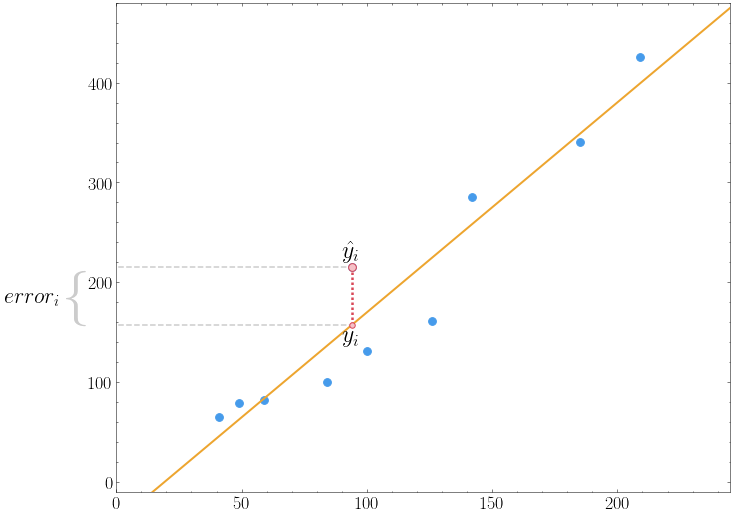
\includegraphics[width=10cm]{images/state-of-art/cost-function/error_function.png}
    \caption{Error de una regresión para el dato $i$}
    \label{fig:error_regression}
\end{figure}


En una red se necesita conocer el error de la capa y no el error de cada neurona. Para ello se aplicará alguna función que reciba un vector como entrada (los errores de cada neurona en una capa) y un único valor de salida (error de la capa). A continuación se listan algunas de las funciones más usadas\cite{tensorflow2015-whitepaper}:


\begin{itemize}
\item \acrfull{mae} \cite{errors_basics} \label{MAE_loss}: Es la métrica de error de regresión más simple de entender. Se toma el error absoluto de cada dato, para que los errores negativos y positivos no se anulen. Luego se calculará la media aritmética. En realidad, el \acrshort{mae} describe la magnitud típica de los residuos. La ecuación es la siguiente:
\begin{equation}
\centering
    \begin{split}
        \text{\acrshort{mae}} = c_i(y_1, \hat{y_1}) = \frac{1}{n} \sum_{i=1}^n |y_i - \hat{y_i}|
    \end{split}
\end{equation}

\begin{figure}[H]
    \centering
    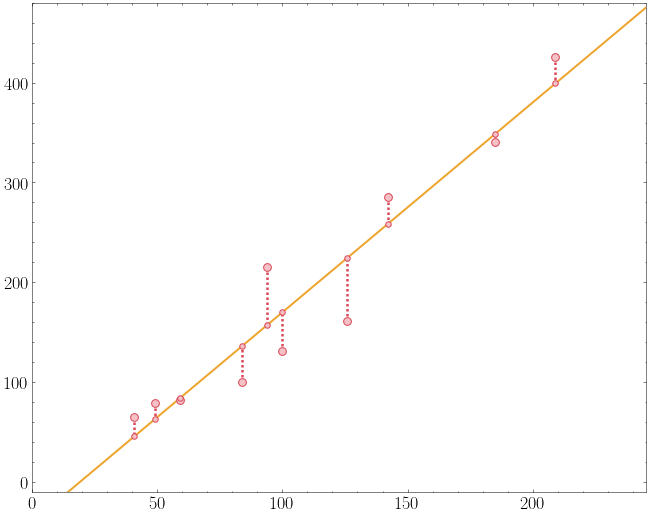
\includegraphics[width=7cm]{images/state-of-art/cost-function/mae.png}
    \caption{Visualización del \acrshort{mae}. El error es la media aritmética de todos los errores.}
    \label{fig:error_mae}
\end{figure}

\item \acrfull{mse} \cite{errors_basics}\label{MSE_loss}: Esta ecuación calcula la media de todos los errores elevados al cuadrado. Elevando al cuadrado se consigue penalizar con mayor intensidad a aquellos puntos que están más alejados de la estimación de la regresión lineal y con menor intensidad a los que se encuentren más cerca. Esta ecuación es muy usada cuando la tarea que se trata de resolver es de tipo regresión. La ecuación es la siguiente:
\begin{equation}
\centering
    \begin{split}
        \text{\acrshort{mse}} = c_i(y_1, \hat{y_1}) &= \frac{1}{n} \sum_{i=1}^n (\sqrt{(\hat{y_i} - y_i)^2}^2) \\
        & = \frac{1}{n} \sum_{i=1}^n (\hat{y_i} - y_i)^2
    \end{split}
\end{equation}

\begin{figure}[H]
    \centering
    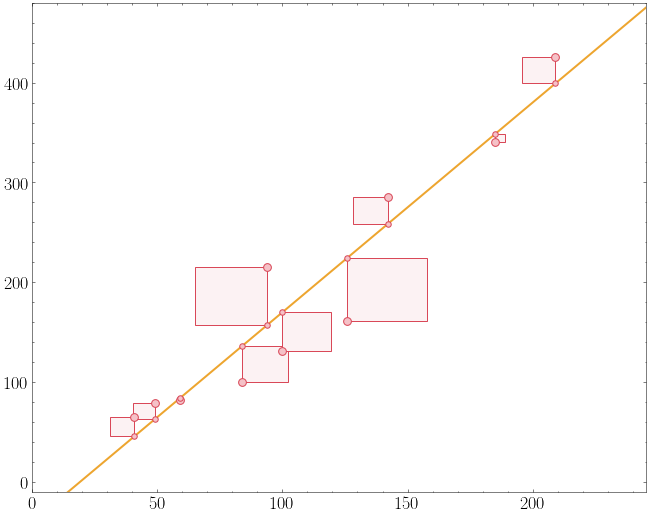
\includegraphics[width=7cm]{images/state-of-art/cost-function/mse.png}
    \caption{Visualización del \acrshort{mse}. El error es la media de las áreas de los cuadrados.}
    \label{fig:error_mae}
\end{figure}

\item \acrfull{rmse} \cite{errors_basics} \label{RMSE_loss}: Esta ecuación es la raíz cuadrada de \acrshort{mse}. Si se compara a nivel de valores, son intercambiables aunque utilizan distinta escala. La ecuación es la siguiente:
\begin{equation}
\centering
    \begin{split}
        \text{\acrfull{rmse}} = \sqrt{\text{\acrshort{mse}}} = \sqrt{\frac{1}{n} \sum_{i=1}^n (\hat{y_i} - y_i)^2}
    \end{split}
\end{equation}

\item \acrfull{msle} \cite{errors_basics} \label{MSLE_loss}: Esta ecuación es parecida a \acrshort{mse}. Se suele utilizar cuando se sabe previamente que los resultados están normalmente distribuidos y no se quiere que los errores grandes sean significativamente más penalizados que los pequeños. La ecuación es la siguiente:
\begin{equation}
\centering
    \begin{split}
        \text{\acrfull{msle}} = c_i(y_1, \hat{y_1}) &= \frac{1}{n} \sum_{i=1}^n (\log{y_i + 1} - \log{\hat{y_i} + 1}) \\
        & = \frac{1}{n} \sum_{i=1}^n \left(\log{\left(\frac{y_i + 1}{\hat{y_i} + 1}\right)}\right)^2
    \end{split}
\end{equation}


\item Pérdida de \textit{Huber}\cite{huber_loss}\label{huber_loss}: Ya se sabe que el Error Medio Cuadrado (\acrshort{mse}) es mejor para aprender los valores atípicos en el conjunto de datos, por otro lado, el Error Medio Absoluto (\acrshort{mae}) es bueno para ignorar los valores atípicos. Pero en algunos casos, los datos que parecen atípicos no molestan y no deberían tener alta prioridad. La pérdida de Huber es una combinación \acrshort{mse} y \acrshort{mae}. Se usará $\delta$ para definir un sesgo para usar \acrshort{mae} o \acrshort{mse}. La ecuación es la siguiente:
\begin{equation}
\centering
    \begin{split}
    \text{Huber\_loss} = c_i(y_1, \hat{y_1}) &= \left\{ 
        \begin{array}{cl} 
            \text{\acrshort{mse}} & \text{si }|\hat{y}-y| \le \delta, \\
            \text{\acrshort{mae}} & \text{e.o.c.}
        \end{array}\right. \\ &= \left\{ 
        \begin{array}{cl} 
            \frac{1}{n} \sum_{i=1}^n (\hat{y_i} - y_i)^2 & \text{si }|\hat{y}-y| \le \delta, \\
            \delta \left(\frac{1}{n} \sum_{i=1}^n |y_i - \hat{y_i}|-\frac{\delta}{n}\right) & \text{e.o.c.}
        \end{array}\right.
    \end{split}
\end{equation}

\begin{figure}[H]
    \centering
    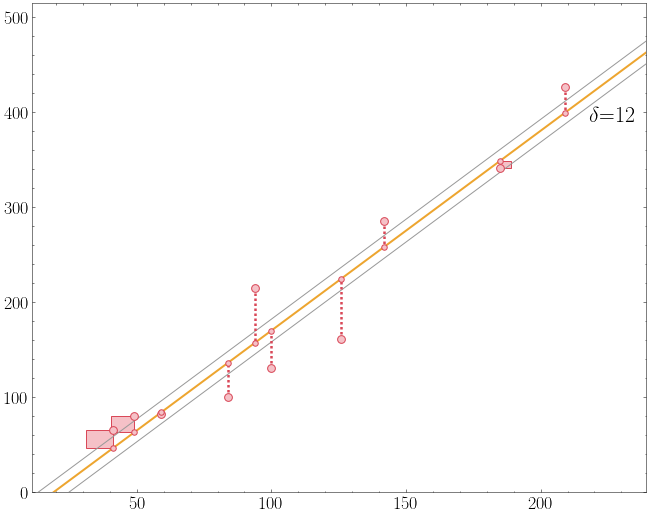
\includegraphics[width=7cm]{images/state-of-art/cost-function/huber.png}
    \caption{Visualización de la pérdida de Huber. Se calcula \acrshort{mse} si $|\hat{y}-y| \le \delta$, en otro caso se calcula \text{\acrshort{mse}}.}
    \label{fig:error_mae}
\end{figure}


\item \acrfull{mape} \cite{errors_basics} \label{MAPE_loss}: Es el porcentaje equivalente de \acrshort{mae}. La ecuación es igual a la de \acrshort{mae}, pero con ajustes para convertir los valores en porcentajes. Permiten ver la distancia entre los resultados del modelo y el resultado real mostrando el dato de manera más fácil de interpretar para los seres humanos. La ecuación es la siguiente:
\begin{equation}
\centering
    \begin{split}
        \text{\acrfull{mape}} = c_i(y_1, \hat{y_1}) &= \frac{100\%}{n} \sum_{i=1}^n \left|\frac{y_i-\hat{y_i}}{y}\right|
    \end{split}
\end{equation}

\begin{figure}[H]
    \centering
    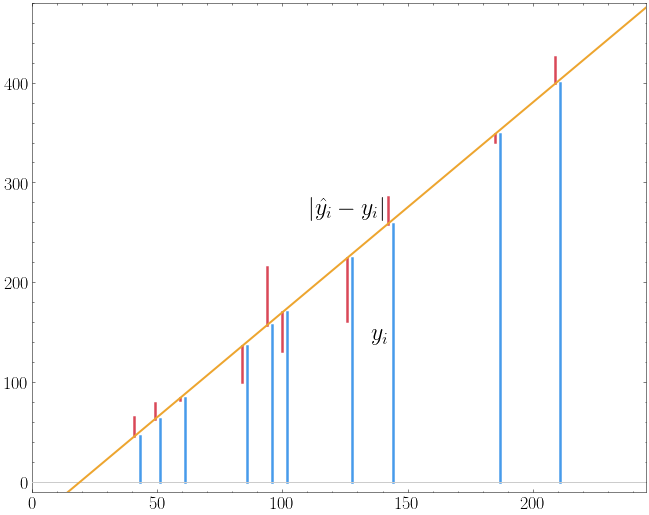
\includegraphics[width=7cm]{images/state-of-art/cost-function/mape.png}
    \caption{Visualización del \acrshort{mape}. El error es la media de las proporciones de los errores respecto al valor $y$.}
    \label{fig:error_mae}
\end{figure}

\item \acrfull{mpe} \cite{errors_basics} \label{MPE_loss}: Es exactamente que \acrshort{mape}, pero sin el valor absoluto. Dado que los errores positivos y negativos se anulan, no se puede hacer ninguna declaración sobre el rendimiento general de las predicciones del modelo. Sin embargo, si hay más errores negativos o positivos, este sesgo se mostrará en el \acrshort{mpe}. A diferencia del \acrshort{mape} y del \acrshort{mae}, el \acrshort{mpe} es útil porque permite ver si el modelo sistemáticamente subestima (más errores negativos) o sobreestima (errores positivos). La ecuación es la siguiente:
\begin{equation}
\centering
    \begin{split}
        \text{\acrshort{mpe}} = c_i(y_1, \hat{y_1}) &= \frac{100\%}{n} \sum_{i=1}^n \frac{y_i-\hat{y_i}}{y}
    \end{split}
\end{equation}

\begin{figure}[H]
    \centering
    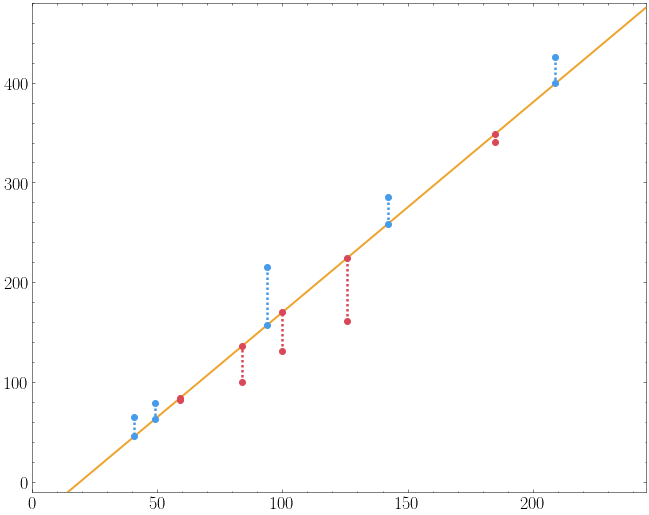
\includegraphics[width=7cm]{images/state-of-art/cost-function/mpe.png}
    \caption{Visualización del \acrshort{mpe}. Muestra la cantidad de errores que son positivos y la cantidad que son negativos.}
    \label{fig:error_mae}
\end{figure}


\item Pérdida de entropía cruzada: Se utiliza explícitamente para comparar una probabilidad de "verdad fundamental" ($y$ u "objetivos") y alguna distribución predicha ($\hat{y}$ o "predicciones"). Tiene como objetivo calcular la media de las probabilidades de que un valor pertenece a una clase o a otra, por lo que es muy útil para problemas de clasificación. Es muy usada cuando se usa la función de activación \textit{softmax}, puesto que esta, también trabaja con probabilidades.
\begin{equation}
\centering
    \begin{split}
        c_i(y_1, \hat{y_1}) &= - \sum_i y_{i,j}log(\hat{y_{i,j}})\\
        \text{donde}~j &= \text{Índice de la probabilidad "verdadera"}
    \end{split}
\end{equation}

La probabilidad "verdadera" es un vector con todos los valores a $0$ excepto uno de ellos que tiene el valor igual a $1$. Este tipo de vector es conocido como vector \textit{one-hot}, donde un valor es \textit{hot} si es igual a $1$ o \textit{cold} si es igual a 0. Cuando se comparan los resultados del modelo con un vector \textit{one-hot} usando la entropía cruzada, los valores igual a $0$ no se usan, y la pérdida de logaritmo de la probabilidad del objetivo se multiplica por $1$, haciendo que el cálculo de la entropía cruzada sea relativamente simple. Este es también un caso especial del cálculo de la entropía cruzada, llamado entropía cruzada por categorías. 
\newline

Un ejemplo de un vector \textit{one-hot} sería el siguiente: $[0,1,0,0]$ donde por ejemplo se representarían las siguientes clases: Perro, gato, caballo y elefante. El $1$ representa que el dato dado al modelo representa a un gato. Este tipo de vectores se usan mucho en tareas de clasificación y en \acrfull{nlp}.
\newline

Hay un subtipo denominado pérdida de entropía cruzada binaria. Este tipo de error se puede calcular cuando se intenta clasificar solo con dos tipos: $0$ o $1$. Normalmente se usa como si fuese un valor booleano en un lenguaje de programación. Un \verb|true| si es del tipo A o un \verb|false| si no es del tipo A. Por ejemplo: gato o no gato o en interior o en exterior. La ecuación matemática es la siguiente:
\begin{equation}
\centering
    \begin{split}
        c_{i,j}(y_1, \hat{y_1}) &= (y_{i,j})(-log(\hat{y}_{i,j})) + (1-y_{i,j}) (-log(1 - \hat{y}_{i,j})) \\
        &= -y_{i,j} \cdot log(\hat{y}_{i,j}) - (1 - y_{i,j}) \cdot log(1 - \hat{y}_{i,j})
    \end{split}
\end{equation}


\end{itemize}

